\documentclass[CT4S-EN-RU]{subfiles}

\begin{document}

\section{\caseENGRUS{Other notions in $\Set$}{ / }{Другие понятия в $\Set$}}

\begin{blockENG}
In this section we discuss some left-over notions in the category of Sets.
\end{blockENG}

\begin{blockRUS}
В данном разделе мы обсудим некоторые из оставшихся понятий в категории множеств. 
\end{blockRUS}

%%%% Subsection %%%%

\subsection{\caseENGRUS{Retractions}{ / }{Ретракции}}

\begin{definitionENG}
Suppose we have a function $f\taking X\to Y$ and a function $g\taking Y\to X$ such that $g\circ f=\id_X$. In this case we call $f$ a {\em retract section} and we call $g$ a {\em retract projection}. \index{retraction}
\end{definitionENG}

\begin{definitionRUS}
Предположим, у нас есть функция $f\taking X\to Y$ и функция $g\taking Y\to X$ такие, что $g\circ f=\id_X$. [О подобной ситуации говорят, как о {\em ретракции}.]\index{ретракция} В этом случае мы называем $f$ {\em сечением ретракции}, а $g$ — {\em проекцией ретракции}.
\end{definitionRUS}

\begin{exerciseENG}
Create an olog that includes sets $X$ and $Y$, and functions $f\taking X\to Y$ and $g\taking Y\to X$ such that $g\circ f=\id_X$ but such that $f\circ g\neq\id_Y$; that is, such that $f$ is a retract section but not an isomorphism.
\end{exerciseENG}

\begin{exerciseRUS}
Придумайте олог, содержащий множества $X$ и $Y$, и функции $f\taking X\to Y$ и $g\taking Y\to X$ такие, чтобы $g\circ f=\id_X$, но чтобы $f\circ g\neq\id_Y$; то есть, чтобы $f$ было сечением ретракции, но не изоморфизмом.
\end{exerciseRUS}

%%%% Subsection %%%%

\subsection{\caseENGRUS{Currying}{ / }{Каррирование}}\label{sec:currying}

\begin{blockENG}
Currying is the idea that when a function takes many inputs, we can input them one at a time or all at once. For example, consider the function that takes a material $M$ and an extension $E$ and returns the force transmitted through the material when it is pulled to that extension. This is a function $e\taking \fakebox{a material}\times\fakebox{an extension}\to\fakebox{a force}$. This function takes two inputs at once, but it is convenient to “curry” the second input. Recall that $\Hom_\Set(\fakebox{an extension},\fakebox{a force})$ is the set of theoretical force-extension curves. Currying transforms $e$ into a function $$e'\taking\fakebox{a material}\to\Hom_\Set(\fakebox{an extension},\fakebox{a force}).$$ This is a more convenient way to package the same information.\index{materials!force extension curves}
\end{blockENG}

\begin{blockRUS}
Каррирование — это идея о том, что в случае функции нескольких аргументов мы можем подставлять их в функцию или по одному, или все сразу. Например, рассмотрим функцию, которая берет материал $M$ и величину деформации $E$, и возвращает силу, возникающую в материале, если деформировать его соответствующим образом. Это функция $e\taking \fakebox{материал}\times\fakebox{деформация}\to\fakebox{сила}$. Эта функция принимает два аргумента сразу, однако удобно «каррировать» ее второй аргумент. Напомним, что $\Hom_\Set(\fakebox{деформация},\fakebox{сила})$ это множество всех теоретически возможных зависимостей силы от деформации. Каррирование преобразует $e$ в функцию $$e'\taking\fakebox{материал}\to\Hom_\Set(\fakebox{деформация},\fakebox{сила}).$$ Это более удобный способ «упаковать» ту же самую информацию.\index{материалы!диаграмма деформации}
\end{blockRUS}

\begin{blockENG}
In fact, it may be convenient to repackage this information another way. For any extension, we may want the function that takes a material and returns how much force it can transmit at that extension. This is a function $$e''\taking\fakebox{an extension}\to\Hom_\Set(\fakebox{a material},\fakebox{a force}).$$ 
\end{blockENG}

\begin{blockRUS}
В принципе, удобным может оказаться и «переупаковывание» информации другим способом. Для каждой деформации мы можем получить функцию, которая принимает материал и возвращает силу, возникающую в нем при данной деформации. Так получается функция $$e''\taking\fakebox{деформация}\to\Hom_\Set(\fakebox{материал},\fakebox{сила}).$$ 
\end{blockRUS}

\begin{notationENG}\index{exponentials ! in $\Set$}
Let $A$ and $B$ be sets. We sometimes denote the set of functions from $A$ to $B$ by 
\begin{align}\label{dia:exponential sets}
B^A:=\Hom_\Set(A,B).
\end{align}
\end{notationENG}

\begin{notationRUS}\index{экспоненциальный объект ! в $\Set$}
Пусть $A$ и $B$ — это множества. Мы иногда будем обозначать множество функций из $A$ в $B$ так: 
\begin{align}\label{dia:exponential sets}
B^A:=\Hom_\Set(A,B).
\end{align}
\end{notationRUS}

\begin{exerciseENG}
For a finite set $A$, let $|A|\in\NN$ denote the cardinality of (number of elements in) $A$. If $A$ and $B$ are both finite (including the possibility that one or both are empty), is it always true that $|B^A|=|B|^{|A|}$?
\end{exerciseENG}

\begin{exerciseRUS}
Для конечного множества $A$, пусть $|A|\in\NN$ обозначает мощность (т.е. число элементов в) $A$. Если оба множества $A$ и $B$ —  конечные (включая возможность того, что одно из них или оба пустые), всегда ли будет верно, что $|B^A|=|B|^{|A|}$?
\end{exerciseRUS}

\begin{propositionENG}[Currying]\label{prop:curry}\index{currying}
Let $A$ denote a set. For any sets $X,Y$ there is a bijection 
\begin{align}\label{dia:curry bijection}
\phi\taking\Hom_\Set(X\times A,Y)\To{\iso}\Hom_\Set(X,Y^A).
\end{align}
\end{propositionENG}

\begin{propositionRUS}[Каррирование]\label{prop:curry}\index{каррирование}
Пусть $A$ обозначает множество. Для любых множеств $X,Y$ имеется биекция%
\endnote{
TODO: Термин «биекция» встречается раньше определения. Поменять на «изоморфизм» или переместить определение?
}%
\endnote{
В случае категории множеств (а именно о ней мы сейчас говорим), есть более легкая для восприятия и запоминания формулировка этого изоморфизма: $(A^X)^Y \iso A^{X\times Y}$
}
\begin{align}\label{dia:curry bijection}
\phi\taking\Hom_\Set(X\times A,Y)\To{\iso}\Hom_\Set(X,Y^A).
\end{align}
\end{propositionRUS}

\begin{proofENG}
Suppose given $f\taking X\times A\to Y$. Define $\phi(f)\taking X\to Y^A$ as follows: for any $x\in X$ let $\phi(f)(x)\taking A\to Y$ be defined as follows: for any $a\in A$, let $\phi(f)(x)(a):=f(x,a)$. 

We now construct the inverse, $\psi\taking\Hom_\Set(X,Y^A)\to\Hom_\Set(X\times A,Y)$. Suppose given $g\taking X\to Y^A$. Define $\psi(g)\taking X\times A\to Y$ as follows: for any pair $(x,a)\in X\times A$ let $\psi(g)(x,a):=g(x)(a)$. 

Then for any $f\in\Hom_\Set(X\times A,Y)$ we have $\psi\circ\phi(f)(x,a)=\phi(f)(x)(a)=f(x,a)$, and for any $g\in\Hom_\Set(X,Y^A)$ we have $\phi\circ\psi(g)(x)(a)=\psi(g)(x,a)=g(x)(a)$, Thus we see that $\phi$ is an isomorphism as desired.
\end{proofENG}

\begin{proofRUS}
Предположим, дана функция $f\taking X\times A\to Y$. Определим $\phi(f)\taking X\to Y^A$ таким образом: для любого $x\in X$ возьмем $\phi(f)(x)\taking A\to Y$, определенную так: для любого $a\in A$, положим $\phi(f)(x)(a):=f(x,a)$. 

Теперь сконструируем обратное отображение, $\psi\taking\Hom_\Set(X,Y^A)\to\Hom_\Set(X\times A,Y)$.  Предположим, дана функция $g\taking X\to Y^A$. Определим $\psi(g)\taking X\times A\to Y$ так: для любой пары $(x,a)\in X\times A$ положим $\psi(g)(x,a):=g(x)(a)$. 

Тогда для любой $f\in\Hom_\Set(X\times A,Y)$ получим $\psi\circ\phi(f)(x,a)=\phi(f)(x)(a)=f(x,a)$, и для любой $g\in\Hom_\Set(X,Y^A)$ выполняется $\phi\circ\psi(g)(x)(a)=\psi(g)(x,a)=g(x)(a)$. Таким образом, мы видим, что $\phi$ — изоморфизм, как и требовалось.
\end{proofRUS}

\begin{exerciseENG}
Let $X=\{1,2\}, A=\{a,b\}$, and $Y=\{x,y\}$. 
\sexc\label{part:three distinct} Write down three distinct elements of $L:=\Hom_\Set(X\times A,Y)$. 
\item Write down all the elements of $M:=\Hom_\Set(A,Y)$. 
\item For each of the three elements $\ell\in L$ you chose in part (\ref{part:three distinct}), write down the corresponding function $\phi(\ell)\taking X\to M$ guaranteed by Proposition~\ref{prop:curry}.
\endsexc
\end{exerciseENG}

\begin{exerciseRUS}
Пусть $X=\{1,2\}, A=\{a,b\}$ и $Y=\{x,y\}$. 
\sexc\label{part:three distinct} Запишите три различных элемента множества $L:=\Hom_\Set(X\times A,Y)$. 
\item Запишите все элементы множества $M:=\Hom_\Set(A,Y)$. 
\item Для каждого из трех элементов $\ell\in L$, выбранных в пункте (\ref{part:three distinct}), запишите соответствующую функцию $\phi(\ell)\taking X\to M$, полученную из Утверждения~\ref{prop:curry}.
\endsexc
\end{exerciseRUS}

\begin{exerciseENG}\label{exc:evaluation}\index{exponentials!evaluation of}
Let $A$ and $B$ be sets. We know that $\Hom_\Set(A,B)=B^A$, so we have a function $\id_{B^A}\taking\Hom_\Set(A,B)\to B^A$. Look at Proposition~\ref{prop:curry}, making the substitutions $X=\Hom_\Set(A,B)$, $Y=B$, and  $A=A$. Consider the function $$\phi^\m1\taking\Hom_\Set(\Hom_\Set(A,B),B^A)\to\Hom_\Set(\Hom_\Set(A,B)\times A,B)$$ obtained as the inverse of (\ref{dia:curry bijection}). We have a canonical element $\id_{B^A}$ in the domain of $\phi^\m1$. We can apply the function $\phi^\m1$ and obtain an element $ev=\phi^\m1(\id_{B^A})\in\Hom_\Set(\Hom_\Set(A,B)\times A,B)$, which is itself a function, $$ev\taking\Hom_\Set(A,B)\times A\to B.$$ 
\sexc Describe the function $ev$ in terms of how it operates on elements in its domain. 
\item Why might one be tempted to denote this function by $ev$?
\endsexc
\end{exerciseENG}

\begin{exerciseRUS}\label{exc:evaluation}\index{экспоненциальный объект!вычисление}
Пусть $A$ и $B$ — это множества. Известно, что $\Hom_\Set(A,B)=B^A$, так что имеется функция $\id_{B^A}\taking\Hom_\Set(A,B)\to B^A$. Взглянем на Утверждение~\ref{prop:curry}, сделав подстановки $X=\Hom_\Set(A,B)$, $Y=B$ и  $A=A$. Рассмотрим функцию $$\phi^\m1\taking\Hom_\Set(\Hom_\Set(A,B),B^A)\to\Hom_\Set(\Hom_\Set(A,B)\times A,B)$$, полученную как обратную к (\ref{dia:curry bijection}). В области определения $\phi^\m1$ имеется канонический элемент $\id_{B^A}$. Мы можем применить функцию $\phi^\m1$ и получить элемент $ev=\phi^\m1(\id_{B^A})\in\Hom_\Set(\Hom_\Set(A,B)\times A,B)$, который сам является функцией, $$ev\taking\Hom_\Set(A,B)\times A\to B.$$ 
\sexc Опишите функцию $ev$ в терминах того, как она действует на элементах своей области определения. 
\item Что побудило нас назвать функцию $ev$?%
\endnote{
На английском это сокращение от {\em evaluate} — вычислять, рассчитывать, оценивать.
}
\endsexc
\end{exerciseRUS}

\begin{blockENG}
If $n\in\NN$ is a natural number, recall from (\ref{dia:underline n}) that there is a nice set $\ul{n}=\{1,2,\ldots,n\}$. If $A$ is a set, we often make the abbreviation 
\begin{align}\label{dia:exponential abbrev}
A^n:=A^{\ul{n}}.
\end{align}
\end{blockENG}

\begin{blockRUS}
Если $n\in\NN$ — это натуральное число, напомним (см.~\ref{dia:underline n}), что имеется замечательное множество $\ul{n}=\{1,2,\ldots,n\}$. Если $A$ — это множество, мы часто используем сокращенную запись
\begin{align}\label{dia:exponential abbrev}
A^n:=A^{\ul{n}}.
\end{align}
\end{blockRUS}

\begin{exerciseENG}\label{exc:two R2s}
In Example~\ref{ex:R2} we said that $\RR^2$ is an abbreviation for $\RR\times\RR$, but in (\ref{dia:exponential abbrev}) we say that $\RR^2$ is an abbreviation for $\RR^{\ul{2}}$. Use Exercise~\ref{exc:generator for set}, Proposition~\ref{prop:curry}, Exercise~\ref{exc:coprod}, and the fact that 1+1=2, to prove that these are isomorphic, $\RR^{\ul{2}}\iso\RR\times\RR$.

(The answer to Exercise~\ref{exc:generator for set} was $A=\singleton$: i.e. $\Hom_\Set(\singleton,X)\iso X$ for all $X$.)
\end{exerciseENG}

\begin{exerciseRUS}\label{exc:two R2s}
В Примере~\ref{ex:R2} мы уже сказали, что $\RR^2$ — это сокращенная запись для $\RR\times\RR$, однако теперь в (\ref{dia:exponential abbrev}) говорим, что $\RR^2$ — это сокращенная запись для $\RR^{\ul{2}}$. Используя Упражнение~\ref{exc:generator for set}, Утверждение~\ref{prop:curry}, Упражнение~\ref{exc:coprod} и тот факт, что 1+1=2, докажите, что эти два определения изоморфны, т.е. $\RR^{\ul{2}}\iso\RR\times\RR$.

(Ответом к Упражнению~\ref{exc:generator for set} является [любое множество с единственным элементом] $A=\singleton$: т.е. $\Hom_\Set(\singleton,X)\iso X$ для всех $X$.)
\end{exerciseRUS}

%%%% Subsection %%%%

\subsection{\caseENGRUS{Arithmetic of sets}{ / }{Арифметика множеств}}\label{sec:arithmetic of sets}

\begin{blockENG}
Proposition~\ref{prop:arithmetic of sets} summarizes the properties of products, coproducts, and exponentials, and shows them all in a familiar light, namely that of arithmetic. In fact, one can think of the natural numbers as literally being the isomorphism classes of finite sets — that's what they are used for in counting. Consider the standard procedure for counting the elements of a set $S$, say cows in a field: one points to an element in $S$ and simultaneously says “1”, points to another element in $S$ and simultaneously says “2”, and so on until finished. This procedure amounts to nothing more than creating an isomorphism (one-to-one mapping) between $S$ and some set $\ul{n}$. 
\end{blockENG}

\begin{blockRUS}
Утверждение~\ref{prop:arithmetic of sets} [см. ниже] подводит итог свойствам произведений, копроизведений и экспоненциальных объектов, и представляет их все в знакомом виде, а именно — в виде арифметики. В принципе, можно думать о натуральных числах буквально как о классах изоморфизма конечных множеств — ведь именно так они используются при счете. Рассмотрим стандартную процедуру подсчета элементов множества $S$, скажем, коров в поле: некто указывает на элемент $S$ [корову] и одновременно говорит “1”, указывает на другой элемент $S$ [другую корову] и одновременно говорит “2”, и так далее, пока они не закончатся. Эта процедура в целом представляет из себя ничто иное, как построение изоморфизма (отображения один-к-одному) между $S$ и некоторым [стандартным конечным] множеством $\ul{n}$. 
\end{blockRUS}

\begin{blockENG}
Again, the natural numbers are the isomorphism classes of finite sets. Their behavior, i.e. the arithmetic of natural numbers, reflects the behavior of sets. For example the fact that multiplication distributes over addition is a fact about grids of dots as in Example~\ref{ex:grid1}. The following proposition lays out such arithmetic properties of sets.
\end{blockENG}

\begin{blockRUS}
Еще раз: натуральные числа являются классами изоморфизма конечных множеств. Их поведение, т.е арифметика натуральных чисел, отражает поведение множеств. Например, тот факт, что умножение дистрибутивно относительно сложения — это факт о сетках точек из Примера~\ref{ex:grid1}. Следующее утверждение перечисляет подобные арифметические свойства чисел.
\end{blockRUS}

\begin{blockENG}
In this proposition, we denote the coproduct of two sets $A$ and $B$ by the notation $A+B$ rather than $A\sqcup B$. It is a reasonable notation in general, and one that is often used. 
\end{blockENG}

\begin{blockRUS}
В этом утверждении мы обозначаем копроизведение двух множеств $A$ и $B$ при помощи $A+B$, а не $A\sqcup B$. Это достаточно осмысленное обозначение в более общем случае, и его часто используют. 
\end{blockRUS}

\begin{propositionENG}\label{prop:arithmetic of sets}\index{set!arithmetic of}
The following isomorphisms exist for any sets $A,B,$ and $C$ (except for one caveat, see Exercise~\ref{exc:0 to the 0}). 
 
\begin{itemize}
\item $A+\ul{0}\iso A$
\item $A + B\iso B + A$
\item $(A + B) + C \iso A + (B + C)$
\item $A\times\ul{0}\iso\ul{0}$
\item $A\times\ul{1}\iso A$
\item $A\times B\iso B\times A$
\item $(A\times B)\times C \iso A\times (B\times C)$
\item $A\times(B+C)\iso (A\times B)+(A\times C)$
\item $A^{\ul{0}}\iso \ul{1}$
\item $A^{\ul{1}}\iso A$
\item $\ul{0}^A\iso\ul{0}$
\item $\ul{1}^A\iso\ul{1}$
\item $A^{B+C}\iso A^B\times A^C$
\item $(A^B)^C\iso A^{B\times C}$
\end{itemize}
\end{propositionENG}

\begin{propositionRUS}\label{prop:arithmetic of sets}\index{множество!арифметика}
Следующие изоморфизмы существуют для любых множеств $A,B$ и $C$ (с единственным исключением, см. Упражнение~\ref{exc:0 to the 0}). 
 
\begin{itemize}
\item $A+\ul{0}\iso A$
\item $A + B\iso B + A$
\item $(A + B) + C \iso A + (B + C)$
\item $A\times\ul{0}\iso\ul{0}$
\item $A\times\ul{1}\iso A$
\item $A\times B\iso B\times A$
\item $(A\times B)\times C \iso A\times (B\times C)$
\item $A\times(B+C)\iso (A\times B)+(A\times C)$
\item $A^{\ul{0}}\iso \ul{1}$
\item $A^{\ul{1}}\iso A$
\item $\ul{0}^A\iso\ul{0}$
\item $\ul{1}^A\iso\ul{1}$
\item $A^{B+C}\iso A^B\times A^C$
\item $(A^B)^C\iso A^{B\times C}$
\end{itemize}
\end{propositionRUS}

\begin{exerciseENG}\label{exc:0 to the 0}
Everything in Proposition~\ref{prop:arithmetic of sets} is true except in one case, namely that of $$\ul{0}^{\ul{0}}.$$ In this case, we get conflicting answers, because for any set $A$, including $A=\emptyset=\ul{0}$, we have claimed both that $A^{\ul{0}}\iso\ul{1}$ and that $\ul{0}^A\iso\ul{0}.$ 

What is the correct answer for $\ul{0}^{\ul{0}}$, based on the definitions of $\ul{0}$ and $\ul{1}$, given in (\ref{dia:underline n}), and of $A^B$, given in (\ref{dia:exponential sets})?
\end{exerciseENG}

\begin{exerciseRUS}\label{exc:0 to the 0}
В Утверждении~\ref{prop:arithmetic of sets} верно все, за исключением одного случая, а именно того, чему изоморфно $$\ul{0}^{\ul{0}}.$$ Для него мы имеем противоречащие друг другу ответы, поскольку для любого множества $A$, включая $A=\varnothing=\ul{0}$, у нас есть пункты и про $A^{\ul{0}}\iso\ul{1}$, и про $\ul{0}^A\iso\ul{0}.$ 

Каков правильный ответ про $\ul{0}^{\ul{0}}$, основанный на определениях $\ul{0}$ и $\ul{1}$, данном в (\ref{dia:underline n}), и $A^B$, данном в (\ref{dia:exponential sets})?
\end{exerciseRUS}

\begin{exerciseENG}
It is also true of natural numbers that if $a,b\in\NN$ and $ab=0$ then either $a=0$ or $b=0$. Is the analogous statement true of all sets?
\end{exerciseENG}

\begin{exerciseRUS}
Есть такой факт о натуральных числах: если $a,b\in\NN$ и $ab=0$, то либо $a=0$, либо $b=0$. Верно ли аналогичное утверждение обо всех множествах?
\end{exerciseRUS}

\begin{blockENG}
Proposition~\ref{prop:arithmetic of sets} is in some sense about isomorphisms. It says that understanding isomorphisms of sets reduces to understanding natural numbers. But note that there is much more going on in $\Set$ than isomorphisms; in particular there are functions that are not invertible.
\end{blockENG}

\begin{blockRUS}
В некотором смысле Утверждение~\ref{prop:arithmetic of sets} говорит об изоморфности. А именно, о том, что понимание изоморфности множеств сводится к пониманию натуральных чисел. Однако, обратите внимание, что в $\Set$ присутствует гораздо больше отображений, чем одни лишь изоморфизмы; в частности, там имеются необратимые функции.
\end{blockRUS}

\begin{blockENG}
In grade school you probably never saw anything that looked like this:
$$5^3\times 3\too 5$$
And yet in Exercise~\ref{exc:evaluation} we found a function $ev\taking B^A\times A\to B$ that exists for any sets $A,B$. This function $ev$ is not an isomorphism so it somehow does not show up as an equation of natural numbers. But it still has important meaning.%
\footnote{Roughly, the existence of $ev\taking\ul{5}^{\ul{3}}\times\ul{3}\too \ul{5}$ says that given a dot in a $5\times 5\times 5$ grid of dots, and given one of the three axes, you can tell me the coordinate of that dot along that axis.} In terms of mere number, it looks like we are being told of an important function $\ul{575}\to\ul{5}$, which is bizarre. The issue here is precisely the one you confronted in Exercise~\ref{exc:functions are not iso invariant}.
\end{blockENG}

\begin{blockRUS}
В начальной школе вы, скорее всего, никогда не видели ничего похожего на это:
$$5^3\times 3\too 5$$
И все же в Упражнении~\ref{exc:evaluation} мы обнаруживаем функцию $ev\taking B^A\times A\to B$, заданную для любых $A,B$. Эта функция $ev$ не является изоморфизмом, так что непохоже, чтобы она привела к чему-то вроде уравнения в натуральных числах. И все же у нее важный смысл.%
\footnote{Грубо говоря, выделенная $ev\taking\ul{5}^{\ul{3}}\times\ul{3}\too \ul{5}$ говорит о том, что если задана некоторая точка в сетке из $5\times 5\times 5$ точек, а также выделена одна из трех осей, то по таким данным можно определить координату заданной точки по выделенной оси.}
Если ограничиваться числами, это выглядит так, как будто нам сообщают об одной важной функции $\ul{575}\to\ul{5}$, что звучит странно. Эта проблема в точности та же, с которой вы сталкивались в Упражнении~\ref{exc:functions are not iso invariant}.
\end{blockRUS}

\begin{exerciseENG}
Explain why there is a canonical function $\ul{5}^{\ul{3}}\times\ul{3}\too \ul{5}$ but not a canonical function $\ul{575}\to\ul{5}$.
\end{exerciseENG}

\begin{exerciseRUS}
Объясните, как может иметься каноническая функция $\ul{5}^{\ul{3}}\times\ul{3}\too \ul{5}$, но не быть при этом канонических функций $\ul{575}\to\ul{5}$.
\end{exerciseRUS}

\begin{sloganENG}
It is true that a set is isomorphic to any other set with the same number of elements, but don't be fooled into thinking that the study of sets reduces to the study of numbers. Functions that are not isomorphisms cannot be captured within the framework of numbers. 
\end{sloganENG}

\begin{sloganRUS}
Хотя верно, что одно множество изоморфно другому множеству с тем же самым числом элементов, но не дайте себя обмануть мыслям о том, что изучение множеств сводится к изучению чисел. Функции, не являющиеся изоморфизмами, не охватываются аппаратом числовой арифметики. 
\end{sloganRUS}

%%%% Subsection %%%%

\subsection{\caseENGRUS{Subobjects and characteristic functions}{ / }{Подобъекты и характеристические функции}}

\begin{definitionENG}\label{def:power set}
For any set $B$, define the {\em power set of $B$}\index{power set}, denoted $\PP(B)$,\index{a symbol!$\PP$} to be the set of subsets of $B$.
\end{definitionENG}

\begin{definitionRUS}\label{def:power set}
Для любого множества $B$, определим {\em множество-степень $B$}\index{множество-степень}, обозначаемое $\PP(B)$,\index{символ!$\PP$} как множество всех подмножеств $B$.
\end{definitionRUS}

\begin{exerciseENG}\label{exc:size of power sets}~
\sexc How many elements does $\PP(\emptyset)$ have? 
\item How many elements does $\PP(\singleton)$ have? 
\item How many elements does $\PP(\{1,2,3,4,5,6\})$ have? 
\item Any idea why they may have named it “power set”?
\endsexc
\end{exerciseENG}

\begin{exerciseRUS}\label{exc:size of power sets}~
\sexc Сколько всего элементов в $\PP(\emptyset)$? 
\item Сколько всего элементов в $\PP(\singleton)$? 
\item Сколько всего элементов в $\PP(\{1,2,3,4,5,6\})$? 
\item Появились ли у вас соображения по поводу названия «множество-степень»?
\endsexc
\end{exerciseRUS}

%% Subsubsection %%

\subsubsection{\caseENGRUS{Simplicial complexes}{ / }{Симплициальные комплексы}}\label{sec:simplicial complex}

\begin{definitionENG}\label{def:simplicial complex}\index{simplicial complex}
Let $V$ be a set and let $\PP(V)$ be its powerset. A subset $X\ss\PP(V)$ is called {\em downward-closed} if, for every $u\in X$ and every $u'\ss u$, we have $u'\in X$. We say that $X$ {\em contains all atoms} if for every $v\in V$ the singleton set $\{v\}$ is an element of $X$. 

A {\em simplicial complex} is a pair $(V,X)$ where $V$ is a set and $X\ss\PP(V)$ is a downward-closed subset that contains all atoms. The elements of $X$ are called {\em simplices} (singular: {\em simplex}).\index{simplex} Any subset $u\ss V$ has a cardinality $|u|$, so we have a function $X\to\NN$ sending each simplex to its cardinality. The set of simplices with cardinality $n+1$ is denoted $X_n$ and each element $x\in X_n$ is called an {\em $n$-simplex}.%
\footnote{It is annoying at first that the set of subsets with cardinality 1 is denoted $X_0$, etc. But this is standard convention because as we will see, $X_n$ will be $n$-dimensional.}
Since $X$ contains all atoms (subsets of cardinality 1), we have $X_0\iso V$, and we may also call the 0-simplices {\em vertices}. We sometimes call the 1-simplices {\em edges}.%
\footnote{The reason we wrote $X_0\iso V$ rather than $X_0=V$ is that $X_0$ is the set of 1-element subsets of $V$. So if $V=\{a,b,c\}$ then $X_0=\{\{a\},\{b\},\{c\}\}$. This is really just pedantry.}

Since $X_0\iso V$, we may denote a simplicial complex $(V,X)$ simply by $X$.
\end{definitionENG}

\begin{definitionRUS}\label{def:simplicial complex}\index{симплициальный комплекс}
Пусть $V$ — это множество, а $\PP(V)$ — его множество-степень. Подмножество $X\ss\PP(V)$ называется {\em замкнутым вниз} если, для каждого $u\in X$ и каждого $u'\ss u$ выполняется $u'\in X$. Мы говорим, что $X$ {\em содержит все атомы}, если для каждого $v\in V$ одноэлементное множество $\{v\}$ является элементом $X$. 

{\em Симплициальный комплекс} это пара $(V,X)$, где $V$ — это множество и $X\ss\PP(V)$ — замкнутоее вниз подмножество, содержащее все атомы. Элементы $X$ называются {\em симплексами}.\index{симплекс} Любое подмножество $u\ss V$ имеет мощность $|u|$, откуда мы получаем функцию $X\to\NN$, переводящую каждый симплекс в его мощность. Множество симплексов мощности $n+1$ обозначается $X_n$, а каждый элемент $x\in X_n$ называется {\em $n$-симплексом}.%
\footnote{Поначалу кажется неудобным, что множество подмножеств мощности 1 обозначается $X_0$, и т.д. Но это стандартное соглашение, поскольку, как мы увидим позже, $X_n$ содержит $n$-мерные симплексы.}
Поскольку $X$ содержит все атомы (подмножества мощности 1), мы получаем $X_0\iso V$; элементы этого множества — 0-симплексы — мы будем называть также {\em вершинами}. Иногда мы также будем называть 1-симплексы {\em ребрами}.%
\footnote{Причина, по которой мы записываем $X_0\iso V$, а не $X_0=V$ — то, что $X_0$ — это [не само $V$, а] множество одноэлементных подмножеств $V$. Так что, если $V=\{a,b,c\}$, то $X_0=\{\{a\},\{b\},\{c\}\}$. На самом деле это всего лишь педантичность.}

Поскольку $X_0\iso V$, [т.е. $V$ полностью определяется по $X$, и поэтому его указание избыточно,] мы можем обозначать симплициальный комплекс $(V,X)$ просто как $X$.
\end{definitionRUS}

\begin{exampleENG}
Let $n\in\NN$ be a natural number and let $V=\ul{n+1}$. Define {\em the $n$-simplex}, denoted $\Delta^n$, to be the simplicial complex $\PP(V)\ss\PP(V)$, i.e. the whole power set, which indeed is downward-closed and contains all atoms. 
\end{exampleENG}

\begin{exampleRUS}
Пусть $n\in\NN$ — натуральное число и $V=\ul{n+1}$. Определим {\em стандартный $n$-симплекс},%
\endnote{
Автор называет $n$-симлексами одновременно и клетки симплициального  комплекса, и простейшие комплексы, порожденные одной клеткой. Чтобы не путать читателя, мы будем добавлять к последним слово {\em стандартный}. Заметим, что стандартный симплекс это не отдельный симплекс, а целый симплициальный комплекс.
}
обозначаемый $\Delta^n$, как симплициальный комплекс $\PP(V)\ss\PP(V)$, т.е. все множество-степень, которое действительно замнуто вниз и содержит все атомы [как это требуется по определению]. 
\end{exampleRUS}

\begin{blockENG}
We can draw a simplicial complex $X$ by first putting all the vertices on the page as dots. Then for every $x\in X_1$, we see that $x=\{v,v'\}$ consists of 2 vertices, so we draw an edge connecting $v$ and $v'$. For every $y\in X_2$ we see that $y=\{w,w',w''\}$ consists of 3 vertices, so we draw a (filled-in) triangle connecting them. All three edges will be drawn too because $X$ is assumed to be downward closed.
\end{blockENG}

\begin{blockRUS}
Мы можем изобразить симплициальный комплекс $X$, нарисовав все вершины в виде точек. Потом для каждого $x\in X_1$ мы видим $x=\{v,v'\}$ состоит из 2 вершин, в результате мы нарисуем ребро, соединяющее $v$ и $v'$. Для каждого $y\in X_2$ мы видим, что $y=\{w,w',w''\}$ состоит из 3 вершин, поэтому нарисуем (сплошной) треугольник, соединяющий их. Все три ребра его уже нарисованы, поскольку $X$ предполагается замкнутым вниз.
\end{blockRUS}

\begin{blockENG}
Thus, the 0-simplex $\Delta^0$, the 1-simplex $\Delta^1$, the 2-simplex $\Delta^2$, and the 3-simplex $\Delta^3$ are drawn here:
\begin{center}
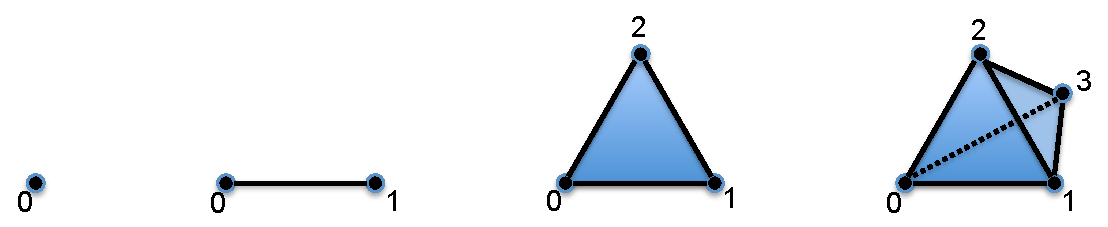
\includegraphics[height=1.1in]{simplices}
\end{center} 
\end{blockENG}

\begin{blockRUS}
Вот, здесь нарисованы стандартные 0-симплекс $\Delta^0$, 1-симплекс $\Delta^1$, 2-симплекс $\Delta^2$ и 3-симплекс $\Delta^3$:
\begin{center}
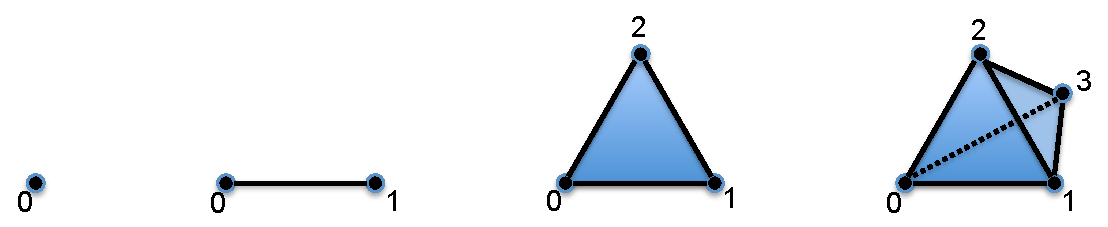
\includegraphics[height=1.1in]{simplices}
\end{center} 
\end{blockRUS}

\begin{blockENG}
The $n$-simplices for various $n$'s are in no way all of the simplicial complexes. In general a simplicial complex is a union or “gluing together” of simplices in a prescribed manner. For example, consider the simplicial complex $X$ with vertices $X_0=\{1,2,3,4\},$ edges $X_1=\{\{1,2\},\{2,3\},\{2,4\}\},$ and no higher simplices $X_2=X_3=\cdots=\emptyset$. We might draw $X$ as follows:
$$\xymatrix{\LMO{1}\ar@{-}[r]&\LMO{2}\ar@{-}[r]\ar@{-}[d]&\LMO{3}\\&\LMO{4}}$$
\end{blockENG}

\begin{blockRUS}
Список стандартных $n$-симплексов для различных $n$ ни в коем случае не исчерпывает все виды симплициальных комплексов. В общем случае симплициальный комплекс является объединением или, вернее, результатом склейки отдельных симплексов предписанным образом. Например, рассмотрим симплициальный комплекс $X$ с вершинами $X_0=\{1,2,3,4\},$ ребрами $X_1=\{\{1,2\},\{2,3\},\{2,4\}\}$ и без симплексов высшей размерности $X_2=X_3=\cdots=\emptyset$. Мы могли бы изобразить $X$ так:
$$\xymatrix{\LMO{1}\ar@{-}[r]&\LMO{2}\ar@{-}[r]\ar@{-}[d]&\LMO{3}\\&\LMO{4}}$$
\end{blockRUS}

\begin{exerciseENG}
Let $X$ be the following simplicial complex, so that $X_0=\{A,B,\ldots,M\}$. 
\begin{center}
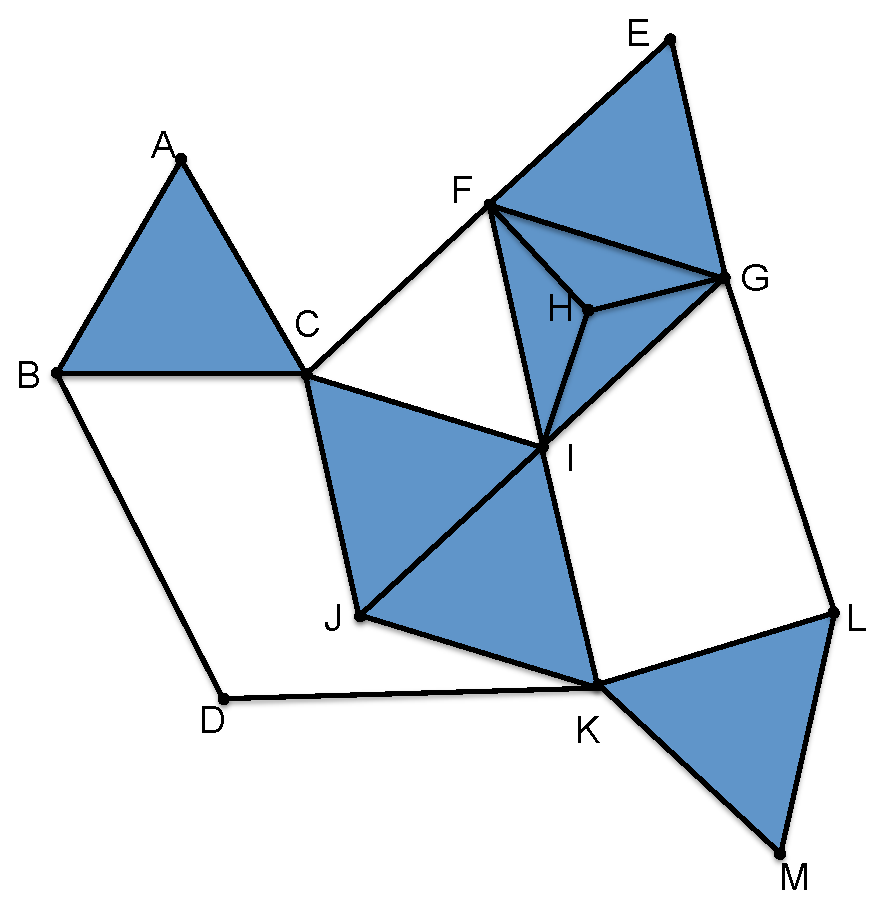
\includegraphics[height=3in]{OlogNetwork5}
\end{center} 
In this case $X_1$ consists of elements like $\{A,B\}$ and $\{D,K\}$ but not $\{D,J\}$. 

Write out $X_2$ and $X_3$ (hint: the drawing of $X$ indicates that $X_3$ should have one element).
\end{exerciseENG}

\begin{exerciseRUS}
Пусть $X$ — это такой симплициальный комплекс, у которого $X_0=\{A,B,\ldots,M\}$. 
\begin{center}
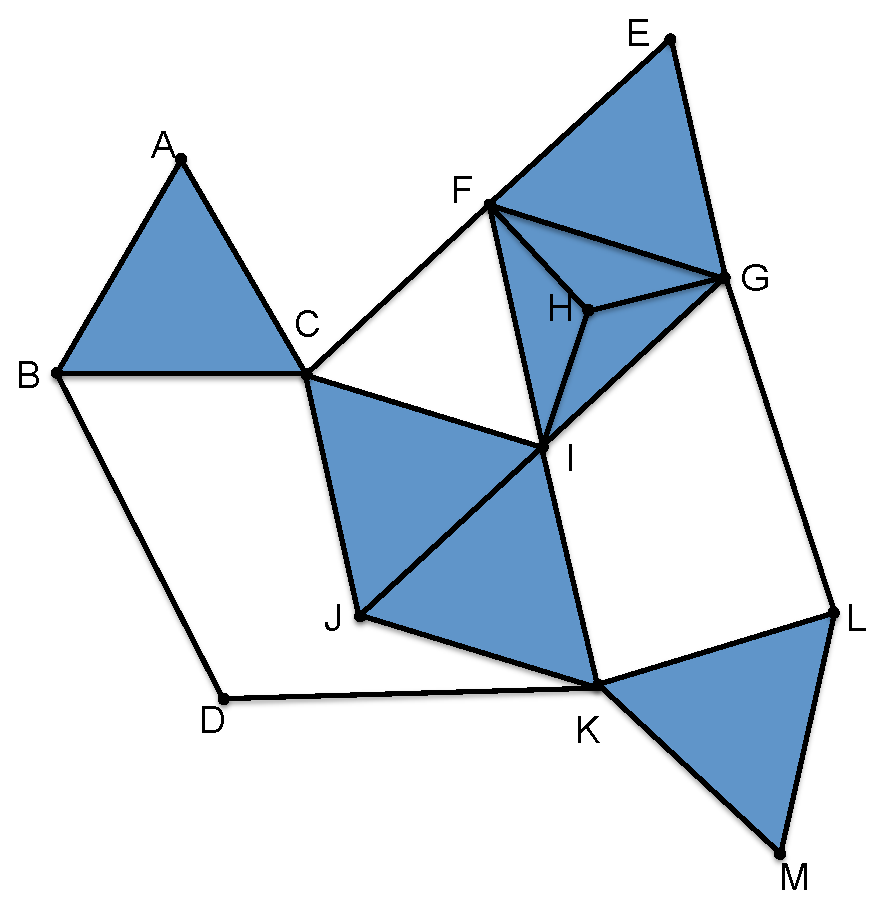
\includegraphics[height=3in]{OlogNetwork5}
\end{center} 
В данном случае $X_1$ состоит из элементов вроде $\{A,B\}$ и $\{D,K\}$, но не $\{D,J\}$. 

Выпишите $X_2$ и $X_3$ (подсказка: изображение $X$ показывает, $X_3$ будет иметь один элемент).
\end{exerciseRUS}

\begin{exerciseENG}
The 2-simplex $\Delta^2$ is drawn as a filled-in triangle with vertices $V=\{1,2,3\}$. There is a simplicial complex $X=\partial\Delta^2$ that would be drawn as an empty triangle with the same set of vertices. 
\sexc Draw $\Delta^2$ and $X$ side by side and make clear the difference.
\item Write down the data for $X$ as a simplicial complex. In other words what are the sets $X_0, X_1, X_2, X_3,\ldots$?
\endsexc
\end{exerciseENG}

\begin{exerciseRUS}
Стандартный 2-симплекс $\Delta^2$ изображается сплошным треугольником с вершинами $V=\{1,2,3\}$. Имеется симплициальный комплекс $X=\partial\Delta^2$, который можно изобразить как пустой треугольник с тем же множеством вершин [и ребер]. 
\sexc Нарисуйте $\Delta^2$ и $X$ рядом друг с другом, чтобы была видна разница между ними.
\item Выпишите данные $X$ как симплициального комплекса. Другими словами, какими будут множества $X_0, X_1, X_2, X_3,\ldots$?
\endsexc
\end{exerciseRUS}

%% Subsubsection %%

\subsubsection{\caseENGRUS{Subobject classifier}{ / }{Классификатор подобъектов}}

\begin{definitionENG}\label{def:subobject classifier}\index{subobject classifier!in $\Set$}
Define the {\em subobject classifier} for $\Set$, denoted $\Omega$\index{a symbol!$\Omega$}, to be the set $\Omega:=\{True,False\}$, together with the function $\singleton\to\Omega$ sending the unique element to $True$.
\end{definitionENG}

\begin{definitionRUS}\label{def:subobject classifier}\index{классификатор подобъектов!в $\Set$}
Определим {\em классификатор подобъектов} в $\Set$, обозначаемый $\Omega$\index{символ!$\Omega$}, как множество $\Omega:=\{True,False\}$ вместе с функцией $\singleton\to\Omega$, переводящей единственный элемент в $True$. 
\end{definitionRUS}

\begin{propositionENG}\label{prop:characteristic function}
Let $B$ be a set. There is an isomorphism $$\phi\taking\Hom_\Set(B,\Omega)\To{\iso}\PP(B).$$
\end{propositionENG}

\begin{propositionRUS}\label{prop:characteristic function}
Пусть $B$ — это множество. Имеется изоморфизм $$\phi\taking\Hom_\Set(B,\Omega)\To{\iso}\PP(B).$$
\end{propositionRUS}

\begin{proofENG}
Given a function $f\taking B\to\Omega$, let $\phi(f)=\{b\in B\|f(b)=True\}\ss B$. We now construct a function $\psi\taking\PP(B)\to\Hom_\Set(B,\Omega)$ to serve as the inverse of $\phi$. Given a subset $B'\ss B$, define $\psi(B')\taking B\to\Omega$ as follows: 
$$\psi(i)(b)=\begin{cases}
True&\tn{ if } b\in B',\\
False&\tn{ if } b\not\in B'.
\end{cases}
$$
One checks easily that $\phi$ and $\psi$ are mutually inverse.
\end{proofENG}

\begin{proofRUS}
Для данной функции $f\taking B\to\Omega$ положим $\phi(f)=\{b\in B\|f(b)=True\}\ss B$. Теперь построим функцию $\psi\taking\PP(B)\to\Hom_\Set(B,\Omega)$, которая будет обратной к $\phi$. Для подмножества $B'\ss B$ определим $\psi(B')\taking B\to\Omega$ следующим боразом: 
$$\psi(i)(b)=\begin{cases}
True,&\tn{ если } b\in B',\\
False,&\tn{ если } b\not\in B'.
\end{cases}
$$
Легко проверить, что $\phi$ и $\psi$ взаимно обратны.
\end{proofRUS}

\begin{definitionENG}[Characteristic function]\index{characteristic function}\index{subset!characteristic function of}
Given a subset $B'\ss B$, we call the corresponding function $B\to\Omega$ the {\em characteristic function of $B'$ in $B$.}
\end{definitionENG}

\begin{definitionRUS}[Характеристичекая функция]\index{характеристическая функция}\index{подмножество!характеристическая функция}
Для данного подмножества $B'\ss B$ назовем соответствующую функцию $B\to\Omega$ {\em характеристической функцией $B'$ в $B$.}
\end{definitionRUS}

\begin{blockENG}
Let $B$ be any set and let $\PP(B)$ be its power set. By Proposition~\ref{prop:characteristic function} there is a bijection between $\PP(B)$ and $\Omega^B$. Since $\Omega$ has cardinality 2, the cardinality of $\PP(B)$ is $2^{|B|}$, which explains the correct answer to Exercise~\ref{exc:size of power sets}.
\end{blockENG}

\begin{blockRUS}
Пусть $B$ — любое множество, а $\PP(B)$ — его множество-степень. Согласно Утверждению~\ref{prop:characteristic function}, имеется биекция между $\PP(B)$ и $\Omega^B$. Покольку $\Omega$ имеется мощность 2, мощность $\PP(B)$ равняется $2^{|B|}$, что является верным ответом к Упражнению~\ref{exc:size of power sets}.
\end{blockRUS}

\begin{exerciseENG}
Let $f\taking A\to\Omega$ denote the characteristic function of some $A'\ss A$, and define $A''\ss A$ to be its complement, $A'':=A-A'$ (i.e. $a\in A''$ if and only if $a\not\in A'$). 
\sexc What is the characteristic function of $A''\ss A$? 
\item Can you phrase it in terms of some function $\Omega\to\Omega$?
\endsexc
\end{exerciseENG}

\begin{exerciseRUS}
Пусть $f\taking A\to\Omega$ обозначает характеристическую функцию некоторого $A'\ss A$; определим $A''\ss A$ как дополнение $A'':=A-A'$ (т.е. $a\in A''$ ттт $a\not\in A'$). 
\sexc Какой будет характеристическая функция $A''\ss A$? 
\item Сможете ли вы выразить это в терминах некоторой функции $\Omega\to\Omega$?
\endsexc
\end{exerciseRUS}

%%%% Subsection %%%%

\subsection{\caseENGRUS{Surjections, injections}{ / }{Сюръекции, инъекции}}

\begin{blockENG}
The classical definition of injections and surjections involves elements, which we give now. But a more robust notion involves all maps and will be given in Proposition~\ref{prop:inj and surj}.
\end{blockENG}

\begin{blockRUS}
Сейчас мы дадим классическое определение инъекций и сюръекций, которое использует элементы. Кроме того ниже, в Утверждении~\ref{prop:inj and surj}, будет представлено более «надежное» определение, использующее только отображения.
\end{blockRUS}

\begin{definitionENG}\label{def:inj,surj,bij}\index{function!injection}\index{function!surjection}\index{function!bijection}
Let $f\taking X\to Y$ be a function. We say that $f$ is {\em surjective} if, for all $y\in Y$ there exists some $x\in X$ such that $f(x)=y$. We say that $f$ is {\em injective} if, for all $x\in X$ and all $x'\in X$ with $f(x)=f(x')$ we have $x=x'$.

A function that is both injective and surjective is called {\em bijective}.
\end{definitionENG}

\begin{definitionRUS}\label{def:inj,surj,bij}\index{функция!инъекция}\index{функция!сюръекция}\index{функция!биекция}
Пусть $f\taking X\to Y$ — это функция. Мы называем $f$ {\em сюръективной}, если для всех $y\in Y$ существует $x\in X$ такой, что $f(x)=y$. Мы называем $f$ {\em инъективной}, если для всех $x\in X$ и $x'\in X$, из $f(x)=f(x')$ следует $x=x'$.

Функция, одновременно инъективная и сюръективная, называется {\em биективной}.
\end{definitionRUS}

\begin{remarkENG}
It turns out that a function that is bijective is always an isomorphism and that all isomorphisms are bijective. We will not show that here, but it is not too hard; see for example \cite[Theorem 5.4]{Big}.
\end{remarkENG}

\begin{remarkRUS}
Оказывается, что биективная функция всегда является изоморфизмом, и что все изоморфизмы биективны. Здесь мы не доказываем этот факт, но делается это не сложно; см., например, \cite[Theorem 5.4]{Big}.
\end{remarkRUS}

\begin{definitionENG}[Monomorphisms, epimorphisms]\label{def:mono, epi in set}\index{epimorphism!in $\Set$}\index{monomorphism!in $\Set$}
Let $f\taking X\to Y$ be a function. 

We say that $f$ is a {\em monomorphism} if for all sets $A$ and pairs of functions $g,g'\taking A\to X$,
$$
\xymatrix{A\ar@/^1pc/[r]^g\ar@/_1pc/[r]_{g'}&X\ar[r]^f&Y}
$$
if $f\circ g=f\circ g'$ then $g=g'$.

We say that $f$ is an {\em epimorphism} if for all sets $B$ and pairs of functions $h,h'\taking Y\to B$, 
$$
\xymatrix{X\ar[r]^f&Y\ar@/^1pc/[r]^h\ar@/_1pc/[r]_{h'}&B}
$$
if $h\circ f=h'\circ f$ then $h=h'$.
\end{definitionENG}

\begin{definitionRUS}[Мономорфизмы, эпиморфизмы]\label{def:mono, epi in set}\index{эпиморфизм!в $\Set$}\index{мономорфизм!в $\Set$}
Пусть $f\taking X\to Y$ — это функция. 

Мы говорим, что $f$ — {\em мономорфизм}, если для всех множеств $A$ и пар функций $g,g'\taking A\to X$,
$$
\xymatrix{A\ar@/^1pc/[r]^g\ar@/_1pc/[r]_{g'}&X\ar[r]^f&Y}
$$
из того, что $f\circ g=f\circ g'$ следует $g=g'$.

Мы говорим, что $f$ — {\em эпиморфизм}, если для всех множеств $B$ и пар функций $h,h'\taking Y\to B$, 
$$
\xymatrix{X\ar[r]^f&Y\ar@/^1pc/[r]^h\ar@/_1pc/[r]_{h'}&B}
$$
из того, что $h\circ f=h'\circ f$ следует $h=h'$.
\end{definitionRUS}

\begin{propositionENG}\label{prop:inj and surj}
Let $f\taking X\to Y$ be a function. Then $f$ is injective if and only if it is a monomorphism; $f$ is surjective if and only if it is an epimorphism.
\end{propositionENG}

\begin{propositionRUS}\label{prop:inj and surj}
Пусть $f\taking X\to Y$ — это функция. Тогда $f$ инъективна, если и только если она является мономорфизмом; $f$ сюръективна, если и только если она является эпиморфизмом.
\end{propositionRUS}

\begin{proofENG}
If $f$ is a monomorphism it is clearly injective by putting $A=\singleton$. Suppose that $f$ is injective and let $g,g'\taking A\to X$ be functions such that $f\circ g=f\circ g'$, but suppose for contradiction that $g\neq g'$. Then there is some element $a\in A$ such $g(a)\neq g'(a)\in X$. But by injectivity $f(g(a))\neq f(g'(a))$, contradicting $f\circ g=f\circ g'$.

Suppose that $f\taking X\to Y$ is an epimorphism and choose some $y_0\in Y$ (noting that if $Y$ is empty then the claim is vacuously true). Let $h\taking Y\to\Omega$ denote the characteristic function of the subset $\{y_0\}\ss Y$ and let $h'\taking Y\to\Omega$ denote the characteristic function of $\emptyset\ss Y$; note that $h(y)=h'(y)$ for all $y\neq y_0$. Then since $f$ is an epimorphism and $h\neq h'$, we must have $h\circ f\neq h'\circ f$, so there exists $x\in X$ with $h(f(x))\neq h'(f(x))$, which implies that $f(x)=y_0$. This proves that $f$ is surjective.

Finally, suppose that $f$ is surjective, and let $h,h'\taking Y\to B$ be functions with $h\circ f=h'\circ f$. For any $y\in Y$, there exists some $x\in X$ with $f(x)=y$, so $h(y)=h(f(x))=h'(f(x))=h'(y)$. This proves that $f$ is an epimorphism.
\end{proofENG}

\begin{proofRUS}
Если $f$ — это мономорфизм, то легко увидеть, что она инъективна, просто подставив $A=\singleton$. Предположим, что $f$ — инъективна и пусть $g,g'\taking A\to X$ — функции такие, что $f\circ g=f\circ g'$; начнем доказывать от противного и предположим, что $g\neq g'$. Тогда имеется некоторый элемент $a\in A$ такой, что $g(a)\neq g'(a)\in X$. Но тогда в силу инъективности $f(g(a))\neq f(g'(a))$, что противоречит условию $f\circ g=f\circ g'$.

Предположим $f\taking X\to Y$ — это эпиморфизм и выберем некоторое $y_0\in Y$ (заметим, что если $Y$ пусто, то утверждение тривиальным образом верно). Пусть $h\taking Y\to\Omega$ обозначает характеристическую функцию подмножества $\{y_0\}\ss Y$, а $h'\taking Y\to\Omega$ — характеристическую функцию $\emptyset\ss Y$; заметим, что $h(y)=h'(y)$ для всех $y\neq y_0$. Тогда, поскольку $f$ — эпиморфизм и $h\neq h'$, выполняется $h\circ f\neq h'\circ f$, так что существует $x\in X$, для которого $h(f(x))\neq h'(f(x))$, откуда следует, что $f(x)=y_0$. Это доказывает, что $f$ сюръективна.

Наконец, предположим, что $f$ сюръективна, а $h,h'\taking Y\to B$ — функции, для которых $h\circ f=h'\circ f$. Для каждого $y\in Y$, существует такой $x\in X$, что $f(x)=y$, поэтому $h(y)=h(f(x))=h'(f(x))=h'(y)$. Это доказывает, что $f$ — эпиморфизм.
\end{proofRUS}

\begin{propositionENG}\label{prop:pb preserve mono}
Let $f\taking X\to Y$ be a monomorphism. Then for any function $g\taking A\to Y$, the top map $f'\taking X\times_YA\to A$ in the diagram
$$
\xymatrix{X\times_YA\ar[r]^-{f'}\ar[d]_{g'}\ullimit&A\ar[d]^g\\X\ar[r]_f&Y}
$$
is a monomorphism.
\end{propositionENG}

\begin{propositionRUS}\label{prop:pb preserve mono}
Пусть $f\taking X\to Y$ — это мономорфизм. Тогда для любой функции $g\taking A\to Y$ верхнее отображение $f'\taking X\times_YA\to A$ в диаграмме
$$
\xymatrix{X\times_YA\ar[r]^-{f'}\ar[d]_{g'}\ullimit&A\ar[d]^g\\X\ar[r]_f&Y}
$$
является мономорфизмом.
\end{propositionRUS}

\begin{proofENG}
To show that $f'$ is a monomorphism, we take an arbitrary set $B$ and two maps $m,n\taking B\to X\times_YA$ such that $f'\circ m=f'\circ n$, denote that function by $p:=f'\circ m\taking B\to A$. Now let $q=g'\circ m$ and $r=g'\circ n$. The diagram looks like this:
$$
\xymatrix{B\ar@<.5ex>[rr]^(.4)m\ar@<-.5ex>[rr]_(.4)n\ar@/^2pc/[rrr]^p\ar@<.5ex>[drr]^(.6)q\ar@<-.5ex>[drr]_(.6)r&&X\times_YA\ar[r]^{f'}\ar[d]_{g'}\ullimit&A\ar[d]^g\\&&X\ar[r]_f&Y}
$$
We have that 
\begin{align*}f\circ q=f\circ g'\circ m=g\circ f'\circ m=g\circ f'\circ n=f\circ g'\circ n=f\circ r\end{align*} 
But we assumed that $f$ is a monomorphism so this implies that $q=r$. By the universal property of pullbacks, Lemma~\ref{lemma:up for fp}, we have $m=n$.
\end{proofENG}

\begin{proofRUS}
Чтобы показать, что $f'$ является мономорфизмом, возьмем произвольное множество $B$ и два отображения $m,n\taking B\to X\times_YA$ такие, что $f'\circ m=f'\circ n$; последнюю функцию обозначим $p:=f'\circ m\taking B\to A$. Теперь положим $q=g'\circ m$ и $r=g'\circ n$. Необходимая диаграмма выглядит так:
$$
\xymatrix{B\ar@<.5ex>[rr]^(.4)m\ar@<-.5ex>[rr]_(.4)n\ar@/^2pc/[rrr]^p\ar@<.5ex>[drr]^(.6)q\ar@<-.5ex>[drr]_(.6)r&&X\times_YA\ar[r]^{f'}\ar[d]_{g'}\ullimit&A\ar[d]^g\\&&X\ar[r]_f&Y}
$$
Выполняются следующие равенства:
\begin{align*}f\circ q=f\circ g'\circ m=g\circ f'\circ m=g\circ f'\circ n=f\circ g'\circ n=f\circ r\end{align*} 
Но, поскольку $f$ — это мономорфизм, отсюда вытекает, что $q=r$. Благодаря универсальному свойству пулбеков, Лемма~\ref{lemma:up for fp}, получаем $m=n$.
\end{proofRUS}

\begin{exerciseENG}
Show, in analogy to Proposition~\ref{prop:pb preserve mono}, that pushouts preserve epimorphisms.
\end{exerciseENG}

\begin{exerciseRUS}
По аналогии с Утверждением~\ref{prop:pb preserve mono} покажите, что пушаут сохраняет эпиморфизмы.
\end{exerciseRUS}

\begin{exampleENG}\label{exc:olog pullbacks}
Suppose an olog has a fiber product square
$$\xymatrix{X\times_ZY\ar[r]^-{g'}\ar[d]_{f'}&Y\ar[d]^f\\X\ar[r]_g&Z}$$ such that $f$ is intended to be an injection and $g$ is any map.%
\footnote{Of course, this diagram is symmetrical, so the same ideas hold if $g$ is an injection and $f$ is any map.} 
In this case, there are nice labeling systems for $f', g'$, and $X\times_ZY$. Namely:
\begin{itemize}
\item “is” is an appropriate label for $f'$, 
\item the label for $g$ is an appropriate label for $g'$,
\item (the label for $X$, then “which”, then the label for $g$, then the label for $Y$) is an appropriate label for $X\times_ZY$.
\end{itemize}

To give an explicit example, 
$$\xymatrix{
\obox{X\times_ZY}{.9in}{a rib which is made by a cow}\LA{rr}{is made by}\LAL{d}{is}&&\obox{Y}{.4in}{a cow}\LA{d}{is}\\
\obox{X}{.3in}{a rib}\LAL{rr}{is made by}&&\obox{Z}{.6in}{an animal}
}
$$
\end{exampleENG}

\begin{exampleRUS}\label{exc:olog pullbacks}
Предположим, в ологе имеется притягивающий квадрат
$$\xymatrix{X\times_ZY\ar[r]^-{g'}\ar[d]_{f'}&Y\ar[d]^f\\X\ar[r]_g&Z}$$ 
такой, что $f$ должна быть инъекцией, а $g$ — любым отображением.%
\footnote{Конечно, эта диаграмма симметрична, так что те же идеи верны и в случае, если $g$ является инъекцией, а $f$ — любым отображением.} 
В таком случае имеется прекрасная система меток для $f', g'$ и $X\times_ZY$. В частности:
\begin{itemize}
\item «является», «это» — это подходящие метки для $f'$, 
\item метка для $g$ подходит и для $g'$,
\item метка (метка $X$, «у которого», метка $g$, метка $Y$) подходит для $X\times_ZY$.
\end{itemize}

В качестве конкретного примера,%
\endnote{TODO переделать, чтобы подходило под «рецепт»} 
$$\xymatrix{
\obox{X\times_ZY}{.9in}{ребро коровы}\LA{rr}{из}\LAL{d}{это}&&\obox{Y}{.4in}{корова}\LA{d}{это}\\
\obox{X}{.3in}{ребро}\LAL{rr}{из}&&\obox{Z}{.6in}{животное}
}
$$
\end{exampleRUS}

\begin{corollaryENG}\label{cor:monos are pullbacks of true}
Let $i\taking A\to X$ be a monomorphism. Then there is a fiber product square of the form 
\begin{align}\label{dia:monos are pbs of true}
\xymatrix{A\ar[r]^{f'}\ar[d]_i\ullimit&\singleton\ar[d]^{True}\\X\ar[r]_f&\Omega.}
\end{align}
\end{corollaryENG}

\begin{corollaryRUS}\label{cor:monos are pullbacks of true}
Пусть $i\taking A\to X$ — это мономорфизм. Тогда имеется притягивающий квадрат вида 
\begin{align}\label{dia:monos are pbs of true}
\xymatrix{A\ar[r]^{f'}\ar[d]_i\ullimit&\singleton\ar[d]^{True}\\X\ar[r]_f&\Omega,}
\end{align}
[который представляет каждый мономорфизм в виде пулбека отображения $True$.]
\end{corollaryRUS}

\begin{proofENG}
Let $X'\ss X$ denote the image of $i$ and let $f\taking X\to\Omega$ denote the characteristic function of $X'\ss X$. Then it is easy to check that Diagram~\ref{dia:monos are pbs of true} is a pullback.
\end{proofENG}

\begin{proofRUS}
Пусть $X'\ss X$ обозначает образ $i$, а $f\taking X\to\Omega$ — характеристическую функцию $X'\ss X$. Тогда легко проверить, что Диаграмма~\ref{dia:monos are pbs of true} является соответствующим притягивающим квадратом.
\end{proofRUS}

\begin{exerciseENG}
Consider the subobject classifier $\Omega$, the singleton $\singleton$ and the map $\singleton\To{True}\Omega$ from Definition~\ref{def:subobject classifier}. Look at diagram~\ref{dia:monos are pbs of true} and in the spirit of Exercise~\ref{exc:olog pullbacks}, come up with a label for $\Omega$, a label for $\singleton$, and a label for $True$. Given a label for $X$ and a label for $f$, come up with a label for $A$, a label for $i$ and a label for $f'$, such that the English smoothly fits the mathematics.
\end{exerciseENG}

\begin{exerciseRUS}
Рассмотрим классификатор подобъектов $\Omega$, синглетон $\singleton$ и отображение $\singleton\To{True}\Omega$ из Определения~\ref{def:subobject classifier}. Взгляните на диаграмму~\ref{dia:monos are pbs of true} и, в духе Упражнения~\ref{exc:olog pullbacks}, предложите метку для $\Omega$, для $\singleton$ и для $True$. Исходя из известных меток для $X$ и для $f$, предложите метку для $A$, для $i$ и для $f'$ так, чтобы естественый язык приближался к математическому.%
\endnote{Опять же, с данной задачей из-за гибкости русского могут быть проблемы...}
\end{exerciseRUS}

%%%% Subsection %%%%

\subsection{\caseENGRUS{Multisets, relative sets, and set-indexed sets}{ / }{Мультимножества, относительные множества, индексированные множества}}

\begin{blockENG}
In this section we prepare ourselves for considering categories other than $\Set$, by looking at some categories related to $\Set$. 
\end{blockENG}

\begin{blockRUS}
В данном разделе мы подготовим себя к изучению отличных от $\Set$ категорий, рассмотрев некоторые категории, связанные с $\Set$. 
\end{blockRUS}

%% Subsubsection %%

\subsubsection{\caseENGRUS{Multisets}{ / }{Мультимножества}}

\begin{blockENG}
Consider the set $X$ of words in a given document. If $WC(X)$ is the wordcount of the document, we will not generally have $WC(X)=|X|$. The reason is that a set cannot contain the same element more than once, so words like “the” might be undercounted in $|X|$. A {\em multiset} is a set in which elements can be assigned a multiplicity, i.e. a number of times they are to be counted. 
\end{blockENG}

\begin{blockRUS}
Рассмотрим множество $X$ слов в заданном документе. Если $WC(X)$ это число слов в документе, мы обычно не получим $WC(X)=|X|$. Причиной является то, что множество не может содержать один и тот же элемент более одного раза, поэтому часто встречающиеся слова не будут правильно учтены в $|X|$. {\em Мультимножество} — это множество, в котором каждому элементу может быть присвоена кратность, т.е. число раз, которое он встретился при подсчете. 
\end{blockRUS}

\begin{blockENG}
But if $X$ and $Y$ are multisets, what is the appropriate type of mapping from $X$ to $Y$? Since every set is a multiset (in which each element has multiplicity 1), let's restrict ourselves to notions of mapping that agree with the usual one on sets. That is, if multisets $X$ and $Y$ happen to be sets then our mappings $X\to Y$ should just be functions.
\end{blockENG}

\begin{blockRUS}
Однако, если $X$ и $Y$ — это мультимножества, то какой же тип подойдет нам в качестве отображений из $X$ в $Y$? Поскольку каждое множество является мультимножеством (в котором каждый элемент имеет кратность 1), давайте ограничимся только теми определениями отображений, что согласованы с обычным понятием отображения между множествами. То есть, если мультимножества $X$ и $Y$ окажутся обычными множествами, то наши отображения $X\to Y$ должны оказаться обычными функциями. 
\end{blockRUS}

\begin{exerciseENG}\label{exc:multiset 1}~
\sexc Come up with some notion of mapping for multisets that generalizes functions when the notion is restricted to sets. 
\item Suppose that $X=(1,1,2,3)$ and $Y=(a,b,b,b)$, i.e. $X=\{1,2,3\}$ with $1$ having multiplicity 2, and $Y=\{a,b\}$ with $b$ having multiplicity 3. What are all the maps $X\to Y$ in your notion?
\endsexc
\end{exerciseENG}

\begin{exerciseRUS}\label{exc:multiset 1}~
\sexc Предложите понятие отображений между мультимножествами, которое превращается в понятие функций, если мы ограничиваемся множествами. 
\item Предположим, что $X=(1,1,2,3)$ и $Y=(a,b,b,b)$, т.е. $X=\{1,2,3\}$, в котором $1$ имеет кратность $2$, а $Y=\{a,b\}$, в котором $b$ имеет кратность $3$. Перечислите все отображения $X\to Y$ согласно вашему определению.
\endsexc
\end{exerciseRUS}

\begin{blockENG}
In Chapter~\ref{chap:categories} we will be getting to the definition of category, and you can test whether your notion of mapping in fact defines a category. Here is my definition of mapping for multisets.
\end{blockENG}

\begin{blockRUS}
В Главе~\ref{chap:categories} будет представлено определение категории, и тогда вы сможете проверить, соответствует ли ваше понятие отображений определению категории. Для сравнения, вот мое определение отображений мультимножеств.
\end{blockRUS}

\begin{definitionENG}\label{def:multiset}\index{multiset}
A {\em multiset} is a sequence $X:=(E,B,\pi)$ where $E$ and $B$ are sets and $\pi\taking E\to B$ is a surjective function. We refer to $E$ as the set of {\em element instances of $X$}, we refer to $B$ as the set of {\em element names of $X$}, and we refer to $\pi$ as the {\em naming function for $X$}. Given an element name $x\in B$, let $\pi^\m1(x)\ss E$ be the preimage; the number of elements in $\pi^\m1(x)$ is called the {\em multiplicity of $x$}.

Suppose that $X=(E,B,\pi)$ and $X'=(E',B',\pi')$ are multisets. A {\em mapping from $X$ to $Y$}, denoted $f\taking X\to Y$, consists of a pair $(f_1,f_0)$ such that $f_1\taking E\to E'$ and $f_0\taking B\to B'$ are functions and such that the following diagram commutes:
\begin{align}\label{dia:multiset map}
\xymatrix{E\ar[r]^{f_1}\ar[d]_{\pi}&E'\ar[d]^{\pi'}\\B\ar[r]_{f_0}&B'.}
\end{align}
\end{definitionENG}

\begin{definitionRUS}\label{def:multiset}\index{мультимножество}
{\em Мультимножество} это последовательность $X:=(E,B,\pi)$, где $E$ и $B$ — это множества, а $\pi\taking E\to B$ — сюръективная функция. Мы будем называть $E$ множеством {\em экземпляров элементов $X$}, $B$ — множеством {\em имен элементов $X$}, а $\pi$ — {\em именующей функцией $X$}. Для заданного имени элемента $x\in B$, пусть $\pi^\m1(x)\ss E$ это прообраз; число элементов в $\pi^\m1(x)$ называется {\em кратностью $x$}.

Предположим, что $X=(E,B,\pi)$ и $X'=(E',B',\pi')$ — это мультимножества. {\em Отображение из $X$ в $Y$}, обозначаемое $f\taking X\to Y$, это пара $(f_1,f_0)$ функций $f_1\taking E\to E'$ и $f_0\taking B\to B'$, для которых следующая диаграмма коммутирует:
\begin{align}\label{dia:multiset map}
\xymatrix{E\ar[r]^{f_1}\ar[d]_{\pi}&E'\ar[d]^{\pi'}\\B\ar[r]_{f_0}&B'.}
\end{align}
\end{definitionRUS}

\begin{exerciseENG}
Suppose that a pseudo-multiset is defined to be almost the same as a multiset, except that $\pi$ is not required to be surjective. 
\sexc Write down a pseudo-multiset that is not a multi-set. 
\item Describe the difference between the two notions in terms of multiplicities. 
\item Complexity of names aside, which do you think is a more useful notion: multiset or pseudo-multisets? 
\endsexc
\end{exerciseENG}

\begin{exerciseRUS}
Предположим, что {\em псевдомультимножество} определено почти так же, как мультимножество, за исключением того, что $\pi$ не обязательно должно быть сурьективным. 
\sexc Запишите псевдомультимножество, не являющееся мультимножеством. 
\item Опишите отличия этих понятий в терминах кратностей элементов. 
\item Если не обращать внимания на сложность названий, то какое понятие, по вашему мнению, более полезно: мультимножество или псевдомультимножество? 
\endsexc
\end{exerciseRUS}

\begin{exerciseENG}
Consider the multisets described in Exercise~\ref{exc:multiset 1}. 
\sexc Write each of them in the form $(E,B,\pi)$, as in Definition~\ref{def:multiset}. 
\item In terms of the same definition, what are the mappings $X\to Y$? 
\item If we remove the restriction that diagram~\ref{dia:multiset map} must commute, how many mappings $X\to Y$ are there?
\endsexc
\end{exerciseENG}

\begin{exerciseRUS}
Рассмотрим мультимножества, описанные в Упражнении~\ref{exc:multiset 1}. 
\sexc Запишите каждое из них в виде $(E,B,\pi)$ согласно Определению~\ref{def:multiset}. 
\item В терминах того же определения, какими будут отображения $X\to Y$? 
\item Если бы мы убрали требование, чтобы диаграмма~\ref{dia:multiset map} коммутировала, сколько всего отображений $X\to Y$ было бы тогда?
\endsexc
\end{exerciseRUS}

%\begin{exampleENG}[Using multisets to approach probability]
%
%Let $S=\{a,b,c,d\}$, and call each element of $S$ a {\em suit}. Let $R=\{1,2,\ldots,13\}$, and call each element of $R$ a {\em rank}. Let $C=S\times R$, and call each element of $C$ a {\em card}. For each $n\in\NN$, let $$A_n=\{f\taking \{1,2,\ldots,n\}\to C\|f \tn{ is injective}\}$$ and call each element of $A_n$ an {\em $n$-card arrangement}. So $A_{52}$ has $52!:=52*51*\cdots*1$ elements and $A_1$ has 52 elements.
%
%The {\em 4-handed poker deal} is the function $A_{52}\to A_5\times A_5\times A_5\times A_5$ given as follows. For each $i\in\{1,2,3,4\}$, let $p_i\taking\{1,2,3,4,5\}\to\{1,2,\ldots,52\}$ be the (injective) function given by the following matrix
%\begin{align}
%\begin{array}{l || l | l | l | l | l}
%i&p_i(1)&p_i(2)&p_i(3)&p_i(4)&p_i(5)\\\hline
%p_1&1&5&9&13&17\\
%p_2&2&6&10&14&18\\
%p_3&3&7&11&15&19\\
%p_4&4&8&12&16&20
%\end{array}
%\end{align}
%Then if $f\taking\{1,2,\ldots,52\}\to C$ is a 52-card arrangement, then $f\circ p_i\taking\{1,2,3,4,5\}\to C$ is a 5-card arrangement, and putting them together we get our 4-handed poker deal.
%
%We could similarly define a $k$-handed poker deal for any $1\leq k\leq 10$. We focus here on $1$-handed poker deals. For any $n\leq 52$, let $\sim_n$ denote the equivalence relation on $A_n$ for which two arrangements are equivalent if one is a permutation (reordering) of the other. Let $H_n=A_n/\sim_n$ be the quotient; we call its elements {\em $n$-card hands}. 
%
%In “5-card poker”, the 5-card hands are classified by patterns of suits and ranks in the cards. More precisely, given a 5-card arrangement $f\taking \{1,2,3,4,5\}\to C$, we consider the compositions with $\pi_1\taking C\to S$ and $\pi_2\taking C\to R$, which we denote $f_S:=\pi_1\circ f$ and $f_R:=\pi_2\circ f$. We are concerned only with the cardinalities of the fibers of $f_S$ and $f_R$. For example if some suit $s\in S$ has $|f_S^\m1(s)|=5$ we say that $f$ (or its equivalence class in $H_5$) is a {\em flush}. If for ranks $r_1,r_2$ we have $|f_R^\m1(r_1)|=2$ and $|f_R^\m1(r_2)|=3$, we call it a {\em full house}. 
%
%\end{exampleENG}

%% Subsubsection %%

\subsubsection{\caseENGRUS{Relative sets}{ / }{Относительные множества}}\label{sec:relative sets}

\begin{blockENG}
Let's continue with our ideas from multisets, but now suppose that we have a fixed set $B$ of names that we want to keep once and for all. Whenever someone discusses a set, each element must have a name in $B$. And whenever someone discusses a mapping, it must preserve the names. For example, if $B$ is the set of English words, then every document consists of an ordered set mapping to $B$ (e.g. $1\mapsto \tn{Suppose}, 2\mapsto\tn{that}, 3\mapsto\tn{we},$ etc.) A mapping from document $A$ to document $B$ would send each word found somewhere in $A$ to the same word found somewhere in $B$. This notion is defined carefully below.
\end{blockENG}

\begin{blockRUS}
Продолжим наши идеи о мультимножествах, но на этот раз предположим, что у нас есть заданное множество имен $B$, которое мы зафиксируем раз и навсегда. Если обсуждается множество, то каждый его элемент должен иметь имя в $B$. Если же обсуждается отображение, то оно должно сохранять имена. Например, если $B$ — это множество слов естественного языка, то каждый документ состоит из упорядоченного множества с отображением его в $B$ (например, $1\mapsto \tn{Предположим}, 2\mapsto\tn{что}, 3\mapsto\tn{мы}$ и т.д.) Отображение документа $A$ в документ $B$ должно переводить каждое слово из $A$ в такое же слово из $B$. Эти понятия подробно определены ниже.
\end{blockRUS}

\begin{definitionENG}[Relative set]\label{def:relative sets}\index{relative set}
Let $B$ be a set. A {\em relative set over $B$}, or simply a {\em set over $B$}, is a pair $(E,\pi)$ such that $E$ is a set and $\pi\taking E\to B$ is a function. A {\em mapping of relative sets over $B$}, denoted $f\taking (E,\pi)\to(E',\pi')$, is a function $f\taking E\to E'$ such that the triangle below commutes, i.e. $\pi=\pi'\circ f$,
$$
\xymatrix@=10pt{E\ar[rr]^f\ar[rdd]_{\pi}&&E'\ar[ldd]^{\pi'}\\\\&B
}
$$
\end{definitionENG}

\begin{definitionRUS}[Относительное множество]\label{def:relative sets}\index{относительное множество}
Пусть $B$ — это множество. {\em Относительное множество над $B$} или просто {\em множество над $B$} — это пара $(E,\pi)$ такая, что $E$ — это множество, а $\pi\taking E\to B$ — функция. {\em Отображение относительных множеств над $B$}, обозначаемое $f\taking (E,\pi)\to(E',\pi')$, — это функция $f\taking E\to E'$ такая, что треугольник ниже коммутирует, т.е. $\pi=\pi'\circ f$,
$$
\xymatrix@=10pt{E\ar[rr]^f\ar[rdd]_{\pi}&&E'\ar[ldd]^{\pi'}\\\\&B
}
$$
\end{definitionRUS}

\begin{exerciseENG}
Given sets $X,Y,Z$ and functions $f\taking X\to Y$ and $g\taking Y\to Z$, we can compose them to get a function $X\to Z$. If $B$ is a set, if $(X,p), (Y,q),$ and $(Z,r)$ are relative sets over $B$, and if $f\taking (X,p)\to (Y,q)$ and $g\taking (Y,q)\to (Z,r)$ are mappings, is there a reasonable notion of composition such that we get a mapping of relative sets $(X,p)\to (Z,r)$? Hint: draw diagrams.
\end{exerciseENG}

\begin{exerciseRUS}
Для данных множеств $X,Y,Z$ и функций $f\taking X\to Y$ и $g\taking Y\to Z$ мы можем образовать композицию, получив функцию $X\to Z$. Допустим, $B$ — это множество, а $(X,p), (Y,q),$ и $(Z,r)$ — относительные множества над $B$ и, кроме того, $f\taking (X,p)\to (Y,q)$ и $g\taking (Y,q)\to (Z,r)$ — отображения; имеется ли тогда осмысленное понятие композиции, которое давало бы в результате отображение относительных множеств $(X,p)\to (Z,r)$? Подсказка: нарисуйте диаграммы.
\end{exerciseRUS}

\begin{exerciseENG}~
\sexc Let $\singleton$ denote a set with one element. What is the difference between sets over $\singleton$ and simply sets?
\item Describe the sets relative to $\emptyset$. How many are there?
\endsexc
\end{exerciseENG}

\begin{exerciseRUS}~
\sexc Пусть $\singleton$ обозначает множество с одним элементом. В чем разница между множествами над $\singleton$ и просто множествами [если она есть]?
\item Опишите относительные множества над $\emptyset$. Сколько их всего?
\endsexc
\end{exerciseRUS}

%% Subsubsection %%

\subsubsection{\caseENGRUS{Indexed sets}{ / }{Индексированные множества}}\label{sec:indexed sets}

\begin{blockENG}
Let $A$ be a set. Suppose we want to assign to each element $a\in A$ a set $S_a$. This is called an $A$-indexed set. In category theory we are always interested in the legal mappings between two different structures of the same sort, so we need a notion of $A$-indexed mappings; we do the “obvious thing”.
\end{blockENG}

\begin{blockRUS}
Пусть $A$ — это множество. Предположим, мы хотим сопоставить каждому элементу $a\in A$ некоторое множество $S_a$. Это называется $A$-индексированным множеством. Поскольку в теории категорий всегда интересуются определенным образом «узаконенными» отображениями между двумя отдельными структурами одного сорта, нам потребуется понятие $A$-индексированных отображений; пойдем очевидным путем. 
\end{blockRUS}

\begin{exampleENG}\label{ex:classroom seats}
Let $C$ be a set of classrooms. For each $c\in C$ let $P_c$ denote the set of people in classroom $c$, and let $S_c$ denote the set of seats (chairs) in classroom $c$. Then $P$ and $S$ are $C$-indexed sets. The appropriate kind of mapping between them respects the indexes. That is, a mapping of multi-sets $P\to S$ should, for each classroom $c\in C$, be a function $P_c\to S_c$.%
\footnote{If we wanted to allow people from any classroom to choose a chair from just any classroom, category theory would tell us to reconsider $P$ and $S$ as sets, forgetting their indices. See Section~\ref{sec:left push}.}
\end{exampleENG}

\begin{exampleRUS}\label{ex:classroom seats}
Пусть $C$ — это множество аудиторий. Для каждого $c\in C$ пусть $P_c$ обозначает множество людей в аудитории $c$, а $S_c$ — множество сидений (стульев) в аудитории $c$. Тогда $P$ и $S$ будут $C$-индексированными множествами. Подходящий вид отображений между ними должен сохранять индексы. Другими словами, отображение $C$-индексированных множеств $P\to S$ [сопоставляющее каждому человеку его сидение] должно для каждой аудитории $c\in C$ быть функцией $P_c\to S_c$.%
\footnote{Если бы мы хотели позволить людям из любой аудитории выбирать стулья из любой [возможно, другой] аудитории, то теория категорий предложила бы нам считать $P$ и $S$ обычными множествами, забыв об их индексах. См. Раздел~\ref{sec:left push}.}
\end{exampleRUS}

\begin{definitionENG}\label{def:indexed sets}\index{indexed set}
Let $A$ be a set. An {\em $A$-indexed set} is a collection of sets $S_a$, one for each element $a\in A$; for now we denote this by $(S_a)_{a\in A}$. If $(S'_a)_{a\in A}$ is another $A$-indexed set, a {\em mapping of $A$-indexed sets from $(S_a)_{a\in A}$ to $(S'_a)_{a\in A}$}, denoted $$(f_a)_{a\in A}\taking(S_a)_{a\in A}\to (S'_a)_{a\in A}$$ is a collection of functions $f_a\taking S_a\to S'_a$, one for each element $a\in A$.
\end{definitionENG}

\begin{definitionRUS}\label{def:indexed sets}\index{индексированное множество}
Пусть $A$ — это множество. {\em $A$-индексированное множество} — это семейство множеств $S_a$, по одному для каждого элемента $a\in A$; мы будем обозначать это при помощи $(S_a)_{a\in A}$. Если $(S'_a)_{a\in A}$ — это другое $A$-индексированное множество, то {\em отображением $A$-индексированных множеств из $(S_a)_{a\in A}$ в $(S'_a)_{a\in A}$}, обозначаемым $$(f_a)_{a\in A}\taking(S_a)_{a\in A}\to (S'_a)_{a\in A},$$ является семейство функций $f_a\taking S_a\to S'_a$, по одному для каждого элемента $a\in A$.
\end{definitionRUS}

\begin{exerciseENG}
Let $\singleton$ denote a one element set. What are $\singleton$-indexed sets and mappings between them?
\end{exerciseENG}

\begin{exerciseRUS}
Пусть $\singleton$ обозначает множество с одним элементом. Какими будут $\singleton$-индексированные множества и отображения между ними?
\end{exerciseRUS}

\begin{exerciseENG}
There is a strong relationship between $A$-indexed sets and relative sets over $A$. What is it?
\end{exerciseENG}

\begin{exerciseRUS}
Имеется тесная связь между $A$-индексированными множествами и относительными множествами над $A$. Какая?
\end{exerciseRUS}

\end{document}
